\setcounter{page}{1}% Start page number with 1
\belowdisplayshortskip=0pt
\renewcommand{\thepage}{\arabic{page}}% Arabic numerals for page counter
\newpage
\chapter{Introduction}
In order to follow the ideas and developments of the upcoming chapters, it is essential to understand some concepts and computational techniques.
In this chapter, we discuss all the necessary knowledge for the proper understanding of this work.
\section{Dark Matter}
Modern cosmology describes the universe as being dominated by two fundamental components: dark energy and matter\footnote{In relativity, mass and energy are equivalent.}.
Dark energy is usually associated with a cosmological constant.

We know of the existence of dark matter entirely from astronomical evidence. In this section we review some of these observations.

\subsection{The missing mass problem in Galaxy Clusters}
The traditional history of dark matter begins in the 1930s with the swiss astronomer Fritz Zwicky\cite{aHistory} \cite{tasiCline}, who measured an unusually high velocity dispersion between the galaxies of the Coma Cluster.
To tackle the problem, Zwicky assumed that the Coma Cluster \tqt{had already reached a mechanically stationary state} \cite{englishZwicky} and such, the virial theorem could be applied.
By counting galaxies, along with assuming that matter is distributed uniformly in the cluster and using Hubble's estimate of the mean mass of a galaxy, Zwicky was able to estimate the potential energy of the Cluster.
Using his estimate of the visible mass and the virial theorem, Zwicky concluded that the velocity dispersion had to be close to $\sqrt{\bar{v^2}} = 80$ km/s.
Nonetheless, the real measurement of the velocity dispersion was $\sqrt{\bar{v^2}} = 1000$ km/s, implying a virial mass about 400 times larger than the visible mass\footnote{This ratio is known as the mass-to-light ratio.}.
Zwicky called the discrepancy between the luminous matter (in the form of visible galaxies which could simply be counted) and the virial matter (obtained from the virial theorem and the high velocity dispersion of the cluster) \tqt{Dark Matter}.

By the late 1950s similar calculations for different clusters had been published. Many of those calculations had very large values for the mass-to-light ratio\cite{schwarzschildSon}, which were consistent with the mass-to-light ratio calculated from the Coma Cluster. The problem of the missing mass seemed to appear in almost every large scale structure in the universe, and by the early 1970s astrophysicist had already disregarded hot gas\cite{meekins} and free hydrogen\cite{penzias} as explanations for the missing mass in Clusters.
Nonetheless, it was still possible that the missing mass problem could be in fact solved by a more refined model of the cluster kinematics, because by then, the missing mass problem had only been observed on Galaxy Clusters and large scale structures.

\subsection{Galaxy Rotation Curves}
A galaxy rotation curve plots the orbital velocity of stars in a galaxy versus their distance to the galaxy centre.
These curves became very informative thanks to the work of the Indian astrophysics Subrahmanyan Chandrasekhar, who proved that the mutual interactions between stars were negligible, so a galaxy could be modeled accurately as a non-interacting system of stars \cite{chandrasekhar}.
Such modeling allows to obtain mass profiles from galaxy rotation curves.
Now, due to photometric measurements, astrophysicist believed that most of  galaxy's mass was overwhelmingly concentrated in the galaxy centre, therefore, it was reasonable to model the galaxy similarly to the solar system.

Consider a star in the galaxy disk with mass $m$ at a distance $r$ from the galaxy centre.
Given that we can disregard the interaction between starts, the sum of forces acting on the object is simply the gravitational attraction towards the centre of the galaxy:
\begin{equation}
\label{heh}
m\frac{v^2}{r} = G \frac{mM}{r^2} \ \text{,}
\end{equation}\\
\vspace{-1mm}with $M$ being the mass enclosed by the star orbit and $v$ being the orbital velocity of the star. Finally, the galaxy rotation curve for such galaxy will be given by
\begin{equation}
v(r) = \sqrt{\frac{GM}{r}} \text{.}
\end{equation}%\vspace{2mm}
Which means that for objects outside of the galaxy disk (but still under the influence of the galaxy gravitational pull) the enclosed mass will be constant regardless of the radius, and thus, the orbital velocity will be proportional to $r^{-1/2}$. With the advent of radio astronomy and the invention of the Image Tube Spectrograph, astronomers were able to measure orbital velocities way beyond the apparent end of the luminous galaxy disks, only to find that the orbital velocity did not decay proportionally to $r^{-1/2}$ but it stayed more or less constant\cite{h21Line} \cite{galactoDistance} \cite{veraFirst}. This behavior can be seen easily in the figure \ref{galaxyCurve}:%\cite{parnovskyCosmology} TODO
\begin{figure}[ht]
    \centering
    %\includegraphics[width=10cm,height =7cm]{Diapositiva1.jpg}
    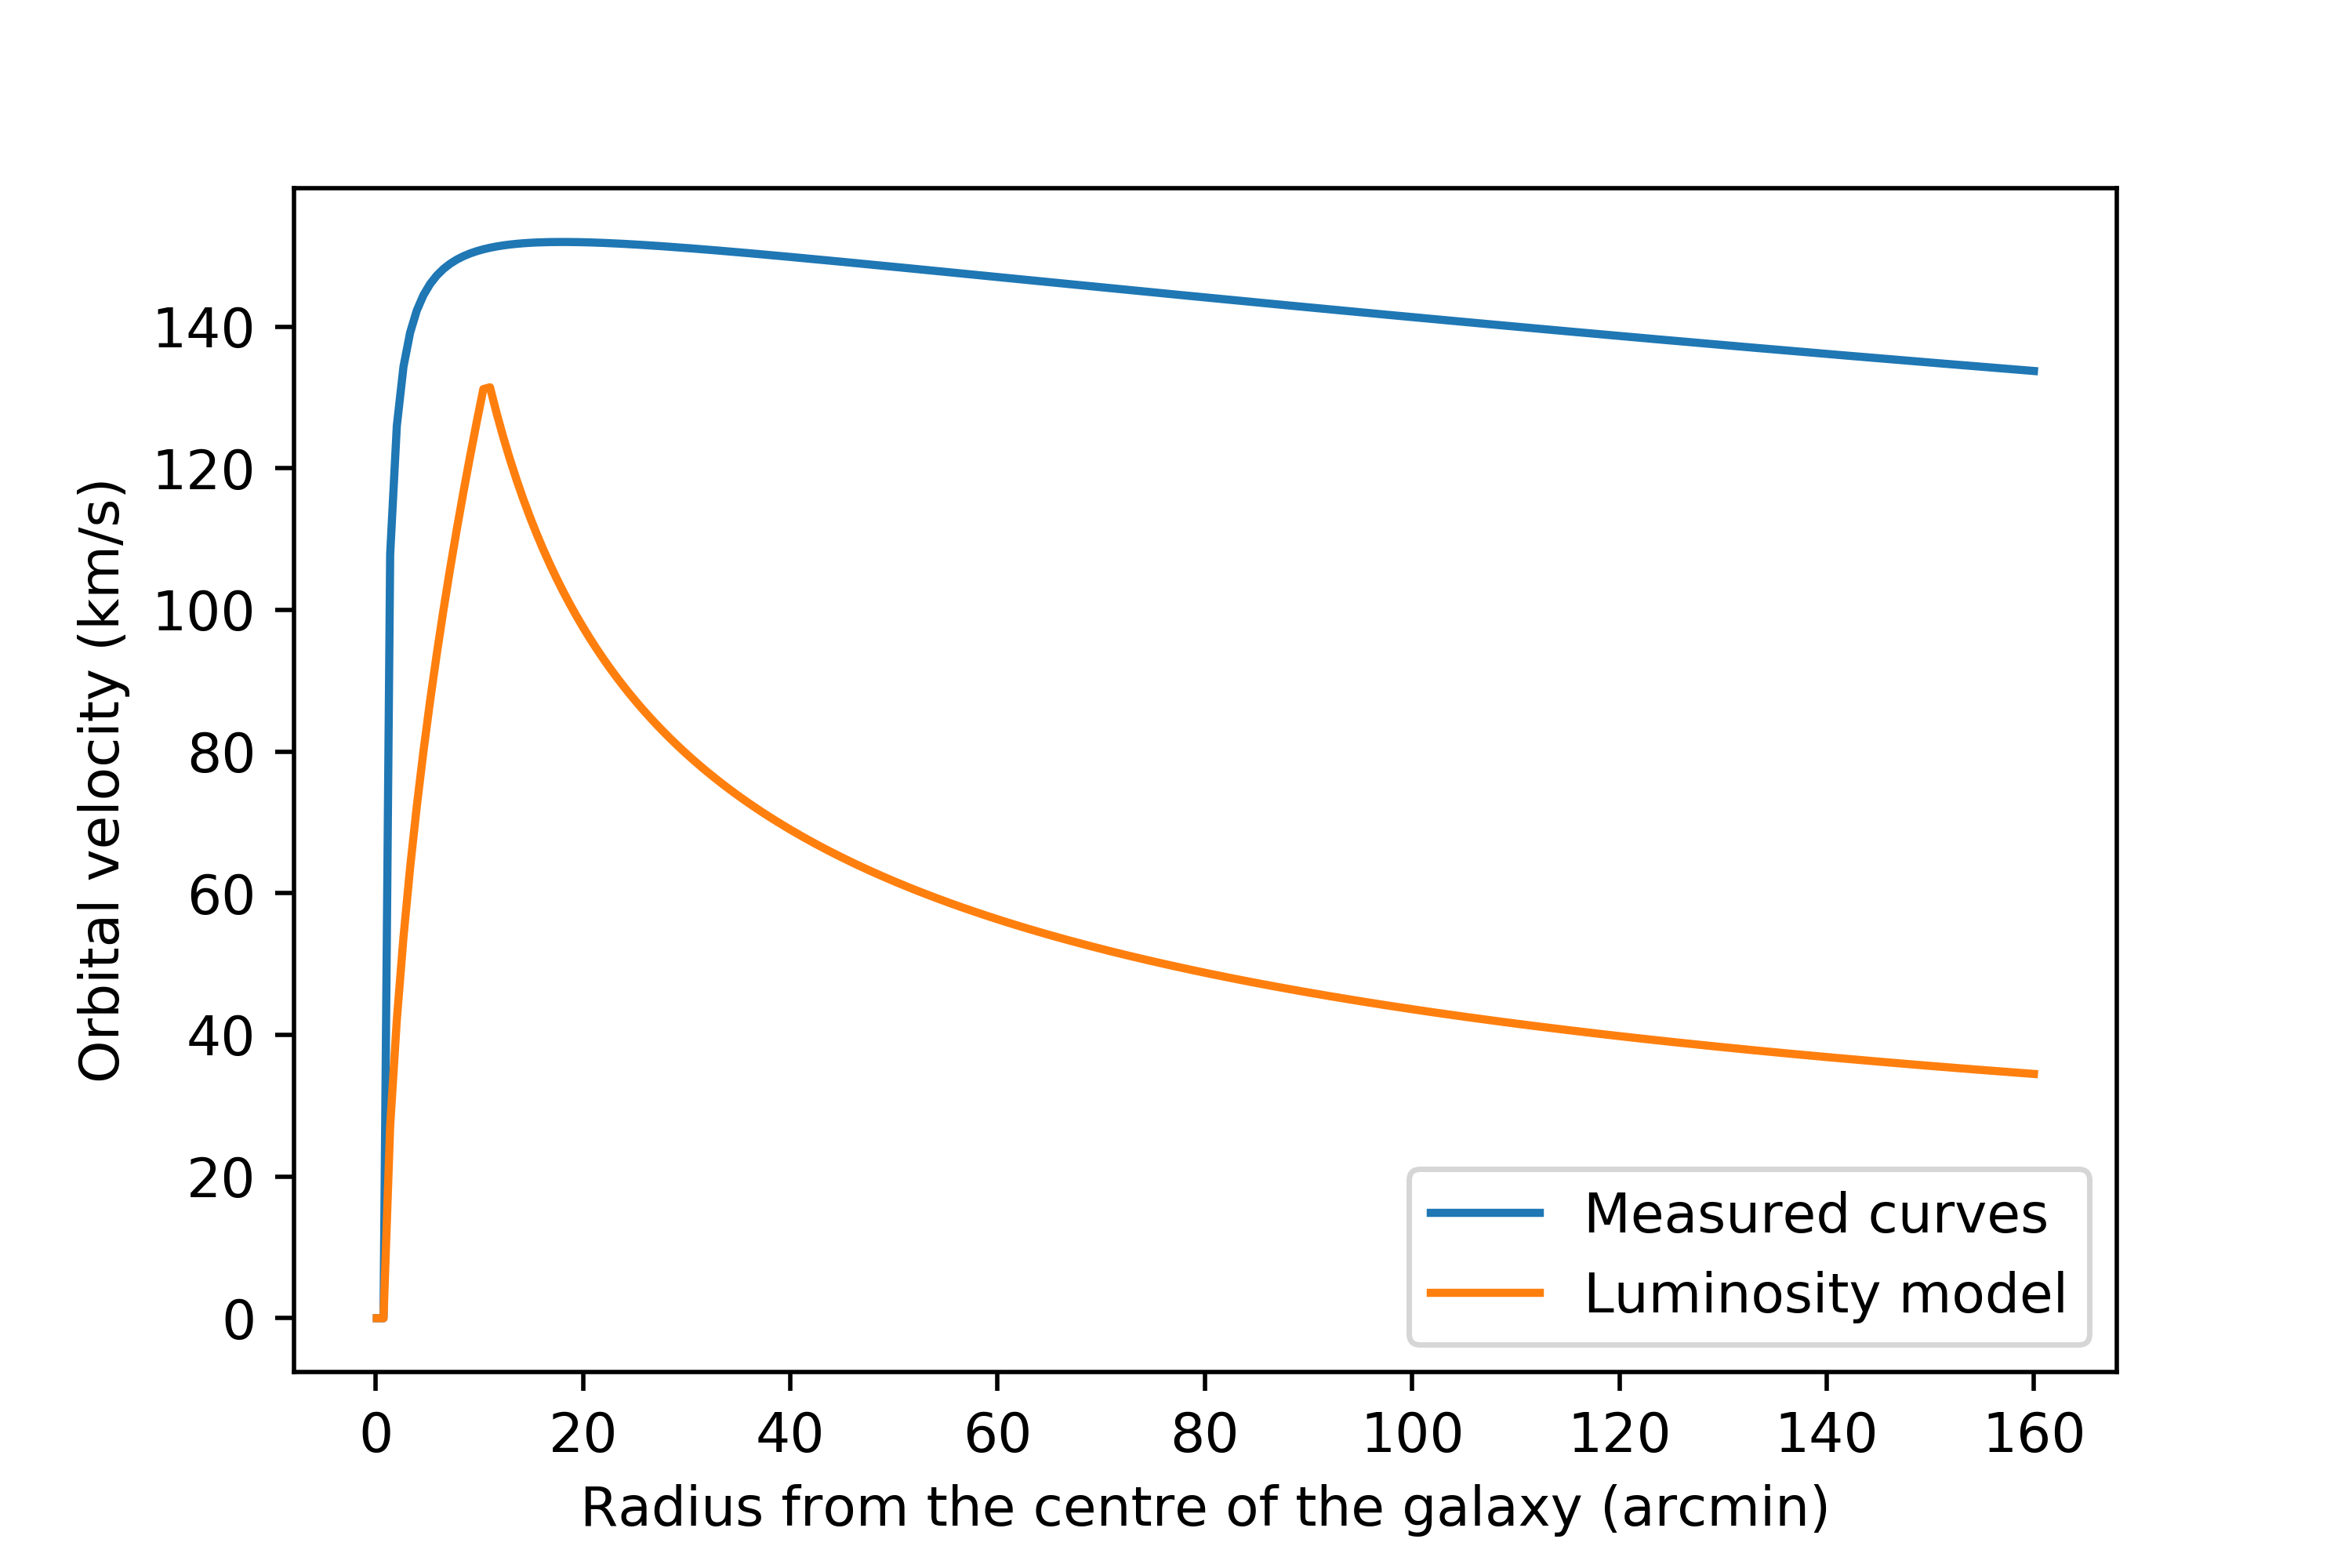
\includegraphics[scale=0.8]{imag/galaxyRotCurv.png}
    \caption{A comparison between the model from photometrical measurements and the curves measured. This curves are simulated and do not correspond to any particular galaxy.}
    \label{galaxyCurve}
\end{figure}

This unexpected velocity profile implied a mass-to-light ratio that increased with distance and also the existence of mass beyond the visible galactic disk\cite{theIsMassOutside}.
The overwhelming amount of high quality galaxy rotation curves measure during the 1970s, let to the acceptance of the dark matter hypothesis in the astrophysical community.

Throughout the use of numerical simulations and the measurement of more galaxy rotation curves during the 1980s and the 1990s, it was concluded that the dark matter density in galaxies was well modeled by the Navarro-Frenk-White (NFW) profile:\cite{FWN}\cite{mariangela}
\begin{equation}
\rho(r) = \frac{\rho_0}{r/r_s(1+r/r_s)^2} \text{.}
\end{equation}
\subsection{The Bullet Cluster}
\label{bulletExplain}
Galaxy clusters have three main constituents: dark matter, intracluster gas (which is mostly ionised hydrogen and helium), and the galaxy themselves.\cite{book:75345}

We can observe the intracluster baryonic matter in the X-ray band thanks to Bremsstrahlung radiation, therefore, by doing photometry in X-ray it is possible to map the baryonic gas distribution in a cluster.
In the case of dark matter, we infer its existence in clusters thanks to the work of Fritz Zwicky and the posterior work in the missing mass problem in galaxy clusters.
Our current estimates place most of the cluster mass in the dark matter component.
By analyzing the gravitational lensing effect (in particular the \emph{weak} gravitational lensing effect) it is possible to map the mass distribution of a galaxy cluster. 
Lastly, we can observe the galaxies in the visual and the infrared band.
They are the only component of a galaxy cluster that can be observed in the visual band.
About 90 percent of the mass of a cluster is dark matter (this is not a surprise since Fritz Zwicky measured mass-to-light ratios of 50 during the 1930s). Of the remaining baryonic matter, the ionized gas mass can represent up to 90$\%$ of the baryonic mass, making galaxies responsible for about 1$\%$ of the total cluster mass.

The object Bullet Cluster (also known as 1E 0657-558) is the aftermath of the collision of two galaxy cluster.
Before the collision, each cluster had its own set galaxies, baryonic gas and dark matter, and the centroid of each constituent coincided with the center of mass of the whole cluster.
During the collision, each constituent reacts differently to the situation:
\begin{itemize}
\item Galaxies, given that they occupy a minuscule fraction of the total volume of the cluster, are essentially collisionless. Two galaxy clusters can collide without any galaxy (or very little galaxies) colliding per se. 
\item Dark matter is also modeled as collisionless, therefore, during the collision of two galaxy clusters, the dark matter components simply pass through, similarly to how Neutrinos constantly cross the Earth without losing a significant amount of energy.
\item The baryonic gas on the other hand is collisional, and its short range interactions are very well described by the Standard Particle Model. During the galaxy cluster collision, the baryonic parts interact and they lose energy through particle collision. This interaction decouples the baryonic gas from the galaxies and dark matter, and, given that we can directly observe the hot gas (thanks to X-ray astronomy), we can measure the separation between the centroid of the hot gas and the centroid of the galaxies.
\end{itemize}

If there was no dark matter, then after the collision the weak lensing mapping of the mass distribution would be very close to the hot gas distribution, because the hot gas would be the dominant mass density in the cluster. If dark matter were to exists, then it would dominate the mass density distribution in the galaxy cluster and the weak lensing mapping would be very similar to the galaxies distribution (because they are also collisionless).

What we observe in the Bullet Cluster is the latter case, in which hot gas decouples from dark matter and galaxies.
By mapping the cluster components and measuring the difference between the centroids, it was concluded that there is a dark matter component in the clusters.
Very accurate measurements and estimates of the centroids show a small collisional nature in the dark matter component, such measurements allows to estimate the \emph{thermally averaged cross-section} of the dark matter particle ( $\crosssection$ ).
Therefore, it is worth exploring the collisional dark matter scenario.

\section{Particle Dark Matter}
So far when talking about dark matter we have talked about an astrophysics problem, however, this problem has also been tackled by the particle physics community. In quantum field theory, particles are modeled as an excitation of space-time fields, and their interactions as interference among those fields. 

The first good candidate for a dark matter particle is the neutrino. 
It is a stable particle, and it does not experience electromagnetic or strong interaction\cite{aHistory}. 
From the measurements of the cosmic microwave background, it is possible to estimate the number of neutrinos that existed in thermal equilibrium during the early universe and the temperature at which they decoupled from the primordial plasma, allowing to define a \emph{thermal relic density}, which is the density of neutrinos (or any specie) at the moment of the decoupling. 
From there, using general relativity, we can study how this density affects the expansion of the universe and place limits on the mass of the particle\cite{Gershtein:1966gg}.
All in all, the neutrino mass was too small to allow for the formation of the large scale structure of the universe. And so, the neutrino was eliminated as a candidate. 

In order to form large scale structure in a dark matter dominated universe, the dark matter particle must decouple as a cold relic\footnote{A particle that decouples from the primordial plasma with a non-relativistic velocity.}. This constrain and the neutrino case (where there is weak and gravitational interaction) lead to the proposal of many \emph{weakly interacting massive particles} (WIMPs) as dark matter particle candidates. This candidates have masses in the GeV regime and a cross section in the same order of magnitude as the weak interaction cross section.  The fact that many extensions of the standard model offered WIMP particles with almost the same thermal relic density as the dark matter particle was known as the WIMP miracle.

There are many other candidates for a dark matter particle, but in the end, every candidate must reproduce the thermal relic density, allow for the formation of halos and large scale structure, and not interact with the electromagnetic field. Any interaction that the dark matter particle has (besides gravitational) implies a cross section $\crosssection$ thus making dark matter collisional. The thermally averaged cross-section $\crosssection$ can be measured using collisions of galaxy clusters such as the Bullet Cluster, once again motivating the study of collisional dark matter.


\section{The Boltzmann Equation}
The Boltzmann equation was originally proposed in 1872 by Ludwig Boltzmann and is used to model the behavior of statistical systems outside of the equilibrium. 
Formally, the Boltzmann equation describes the evolution of the phase space of a typical dark matter particle, such that $\f \dd \vb{r} \dd \vb{v}$ is the probability of finding the dark matter particle in a position between $\vb{r}$ and $\vb{r} + \dd \vb{r}$, with velocity velocity between $\vb{v}$ and $\vb{v} + \dd \vb{v}$.
By multiplying the probability phase space by the mass of a dark matter particle and the number of particles enclosed in the volume of interest ($n$), we can use the Boltzmann equation to describe the phase space mass density of a fluid, instead of the phase space probability of a single particle.
In this work we are interested in the phase space mass density of a dark matter fluid, whose time evolution is described by the Boltzmann equation
\begin{equation}
\pdv{f}{t} + \vb{\dot{x}} \pdv{f}{\vb{x}} + \vb{\dot{v}} \pdv{f}{\vb{v}}  = C[f]  \text{,}
\end{equation}
the left hand side is known as the Liouville operator and the right hand side is known as the \emph{Collisional} operator. The Liouville operator represents the evolution of the system following classical mechanics, without considering short range interaction between particles (the collisions).
The collisional operator is an integral operator that relates the possibility of a collision with the state of the system $\f$. 
In other words, the collisional operator quantifies the effect of the collisions in the phase space evolution.
A complete modeling of the collisional operator requires knowledge of the short range interactions between particles, given that we do not know the short range interaction of a dark matter particle, we must work with approximation schemes. This is going to be expanded in section \ref{bgk}.\vspace{5mm}\\
\vspace{1mm}For a collisionless fluid, the Boltzmann equation becomes the Vlasov equation:
\begin{equation}
\pdv{f}{t} + \vb{\dot{x}} \pdv{f}{\vb{x}} + \vb{\dot{v}} \pdv{f}{\vb{v}}  = 0 \text{.}
\end{equation}
Which simply dictates that the phase space distribution function is constant along the trajectories of the system\cite{integerLatticeDynamics}
\section{Lattice Boltzmann Method}
\label{boltz}
The Lattice-Boltzmann method divides the phase space into a lattice and solving the Boltzmann equation in such lattice.
In each cell of the lattice there is a density which represents the mass of fluid in the position and velocity range correspondent to the cell's location in the lattice.
The main effect of the discretization of the phase space is that we no longer simulate the entire phase space, but a discrete number of velocities and positions, which allows for the use of integer arithmetic. The use of integer arithmetic introduces lattice noise but eliminates the floating point error. In the limit of high resolution, the absence of floating point error and the tendency of the lattice noise towards zero guarantees that the method converges to the continuum solution and makes it a Lagragian, Symplectic and conservative algorithm. 

However, this method has one big drawback. The time evolution of the phase space is calculated using a direct integration scheme, which implies that for a simulation with $N$ spatial dimensions each one having size $n$, we would need to store $n^{2N}$ cell units per timestep. This is in fact a very heavy constrain because most cases of interest are three dimensional. For example, in a three dimensional distribution, if the grid size were to be $64$, then we would need almost 600 Gigabytes of memory just to store the lattice. 
The specifics of implementing a Lattice Boltzmann method are discussed further in section \ref{implementBoltzmann}.



\section{BGK Approximation}
\label{bgk}
The main challenge when solving the Boltzmann equation is the collisional operator. Modeling a collisional operator and solving the subsequent integral is not a straightforward procedure, which is why simpler alternatives have been widely considered.

The Bhatnagar–Gross–Krook approximation was proposed in 1954 \cite{1954PhRv...94..511B} in order to simplify the collision integral.
The approximation operates under the assumption that the large amount of detail involved in the two-body interactions are not likely to significantly influence the macroscopic variables\cite{asinari}.
This is known as an mesoscopic approach, because we disregard the microscopic interactions while preserving the macroscopic properties of the system. 
The scheme ignores the specifics of the two-body interactions but keeps the tendency of the system towards local equilibrium and then global equilibrium.

Local equilibrium is defined by the following condition:
\begin{equation}
C[f_e] = 0\text{.}
\end{equation}
Which simply states that in \emph{local equilibrium}, the collisions do not affect the time derivative of the distribution function. Note that local equilibrium does not mean that the macroscopic variables of the system are constant in space and time, but that the local value of  $\f$ corresponds to the local value of $f_e(\rv)$, for an appropriate equilibrium distribution function $f_e(\rv)$. Finally, the BGK operator can be stated as:
\begin{equation}
C[f] = -\frac{1}{\tau}(\f - f(\rv)) \text{,}
\end{equation}


where $\tau$ is a characteristic relaxation time for the system. In most cases, the equilibrium function obeys the Maxwell-Boltzmann distribution, however, Fermi-Dirac distributions were widely used in the early years of the Lattice Boltzmann methods.
In recent years modified Maxwellians have been proposed to extend the BGK scheme to the quantum realm\cite{2010arXiv1009.3352F} and to include annihilation and creation of particles. The specifics of our implementation of the BGK approximation are discussed in section \ref{metodologiaBGK}.











